\documentclass[12pt, a4paper]{article}

\usepackage[czech]{babel}
\usepackage[IL2]{fontenc}
\usepackage[utf8]{inputenc}
\usepackage{lmodern}  % lepší kvalita PDF

\usepackage[a4paper,top=3cm,bottom=3cm,left=3cm,right=3cm,marginparwidth=1.75cm]{geometry}

\usepackage{graphicx}
\usepackage{titling}
\usepackage{enumitem}
\usepackage{caption}
\usepackage{float}
\usepackage{pdfpages}
\usepackage{verbatim}
\usepackage{amsmath}

\usepackage{pkg-custom-commands}
\usepackage{pkg-url}

% údaje na titulní straně
\title{Cvičení 2}
\def \thesubtitle {KIV/VSS}
\author{Patrik Harag}
\def \theauthoremail {harag@students.zcu.cz}
\def \theauthorid {A18N0084P, nar. 10. května}

\begin{document}

\begin{titlepage}
	\begin{figure}
		
\includegraphics[height=50mm]{img-fav-logo}
	\end{figure}
	
	\centering
	{\large \hspace{1mm} \par} % tady musí být nějaký text jinak nefunguje vertikální odsazení
	\vspace{15ex}
	
	{\huge\bfseries \thetitle \par}
	\vspace{2ex}
	{\scshape\Large \thesubtitle \par}
	\vspace{15ex}
	{\Large\itshape \theauthor \par}
	\vspace{2ex}
	{\texttt{\theauthoremail} \par}
	\vspace{1ex}
	{\texttt{\theauthorid} \par}
	
	\vfill

	{\today\par}
\end{titlepage}

\section*{Zadání}

\paragraph{3.}
Telefonní ústředna je modelována systémem M/M/3 s nulovou délkou fronty (tj. pokud jsou obsazeny všechny (tři) linky, volající nečeká - zavěsí). Průměrná doba trvání hovoru je 2 min a průměrný počet požadavků na spojení je 50/hod. Z modelu určete pravděpodobnost obsazení ústředny (tj. stavu kdy všechny linky jsou obsazené) a pravděpodobnost, že požadavek na spojení bude uspokojen (tj. alespoň jedna linka je volná).

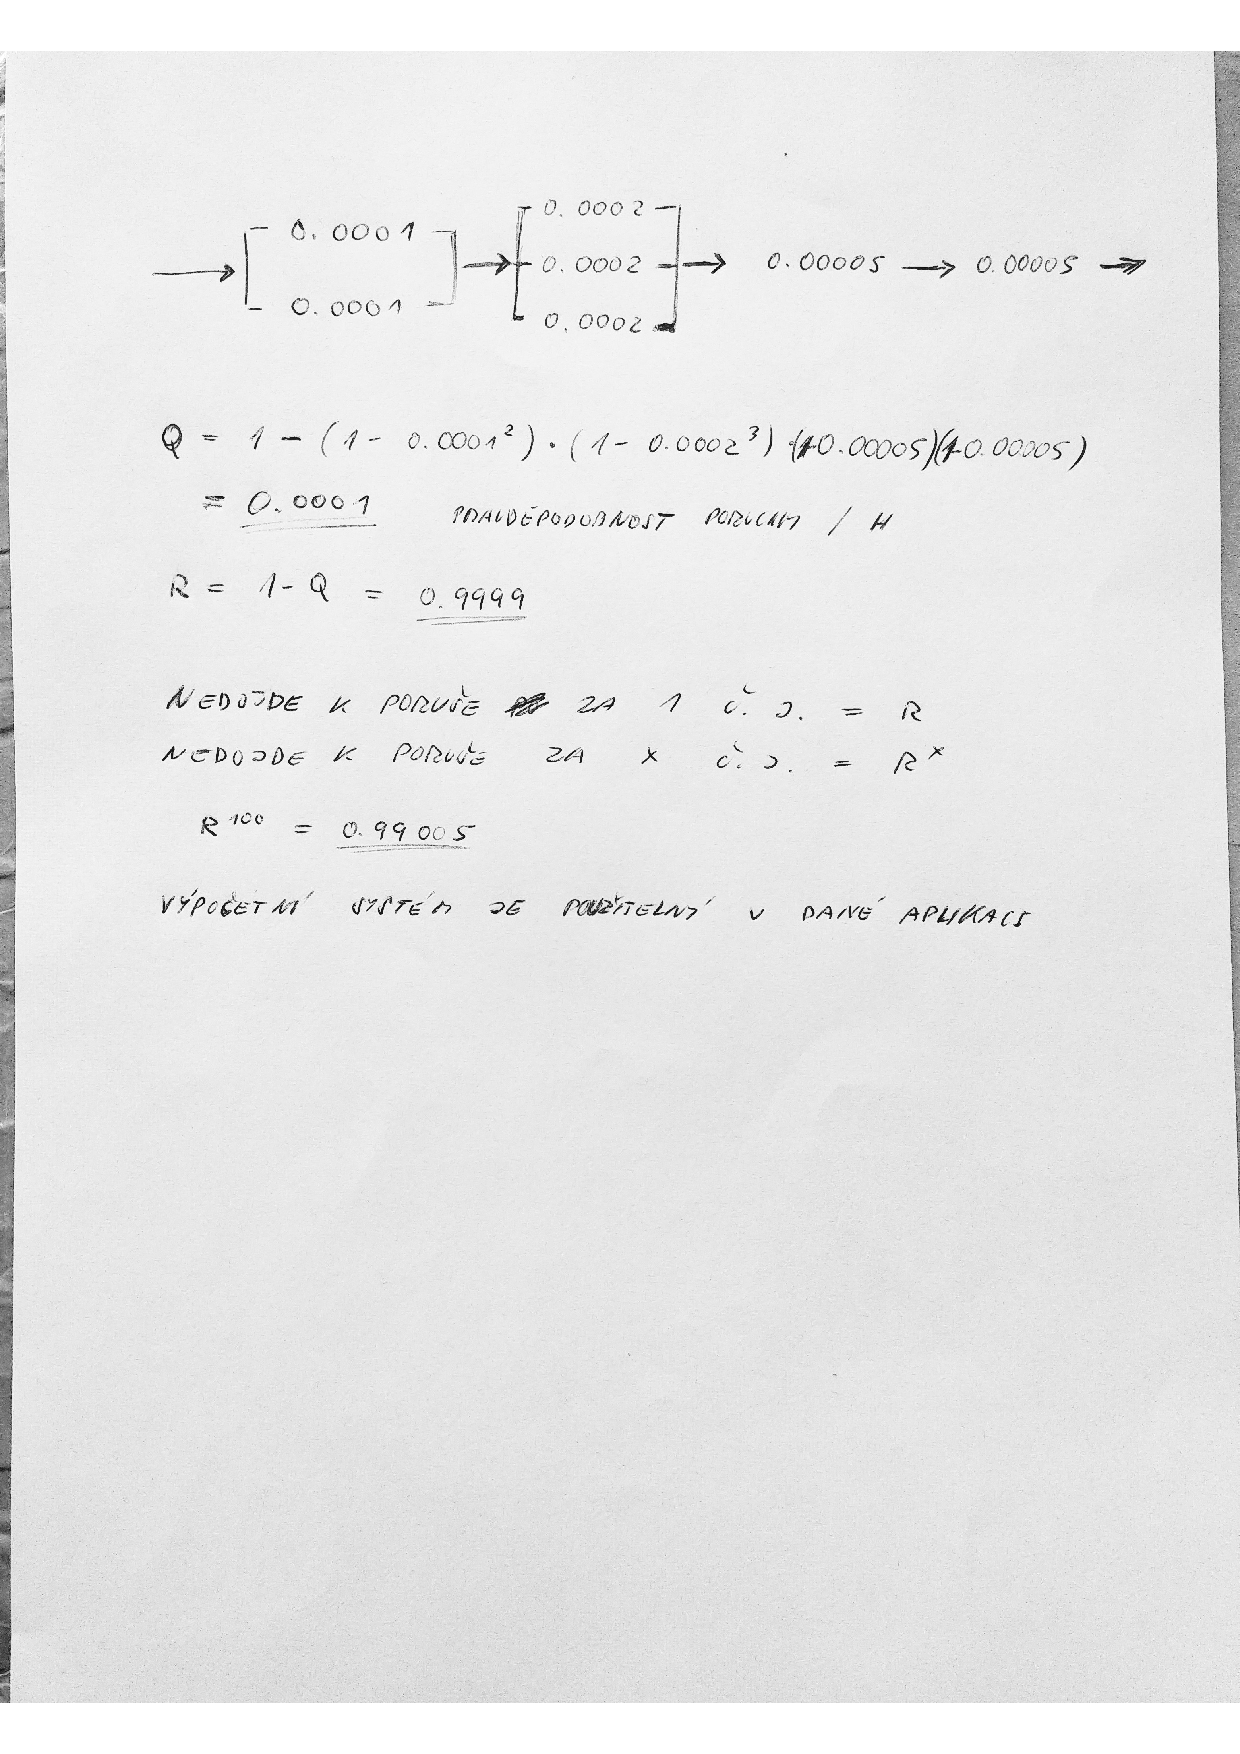
\includepdf[pages={1}]{priklad.pdf}

\end{document}